\section{Introduction}

Atomic chains are a prototype for the study of
molecular electronic systems. Atomic nanowires can be fabricated on
inert surfaces \cite{segovia1999nature,nilius2002science} or in
mechanically controlled break junctions \cite{vanruitenbeek1998mcbj}.
Atomic nanowires are of fundamental scientific interest as they form
electronic one-dimensional systems and for technology they may be viewed
as the limit for metal interconnects in use for nanoelectronics.  Atomic
nanowires are also useful for benchmarking one-dimensional quantum
transport formulations as experiments for these systems provide well
defined and understood conductance values.

Some of the earliest theoretical work with explicit treatment of the
electronic within a quatum transport study of atomic chains is due to
Lang~\cite{Lang1995prb} and this work has served as the model for
subsequent studies in molecular tunnel junctions. In this early work,
jellium electrodes are coupled to metal atom chains and the electronic
structure of the system is treated using \ac{DFT}. The Kohn-Sham states
in \ac{LDA} are treated as quasiparticles and the electron
scattering equations are solved for the case of an external voltage bias
applied to the electrodes. Similar scattering approaches in conjunction
with tight binding Hamiltonians applied to the conductance of molecular
junctions combined with Landauer-B\"uttiker theory for electron transport
\cite{emberlykirczenow1999standingwave,
emberlykirczenow2000molecularwire} have been undertaken. 
Subsequently, similar methods have gained prominence by combining a \ac{DFT}
treatment of the electronic structure with a formal \ac{NEGF} treatment of
transport in open systems. More recently, the {\it GW}
approximation~\cite{hedin1965gw} has been introduced to improve  the
quaisparticle description of atomic scale tunnel junctions beyond a Kohn-Sham
description~\cite{thygesen_rubio,neaton2007amines}.  Use of the
Kohn-Sham energies in the NEGF formulation implies a single determinant
approximation to the many-electron Green's function and similarly the
{\it GW} approximation may be viewed as dynamically screened version of
the Hartree-Fock theory, likewise implying a single determinant
approximation to the many-electron Green's function.  Alternative to
these methods are to use the ideas of exact diagonalization or
configuration interaction in rate equation formulations of electron
transport~\cite{pedersen_many_body_tunneling} or through a many-electron
scattering formulation of the transport problem~\cite{vici2004}. 

In defining models for atomic-scale transport junctions, a partitioning
of the system into semi-infinite electrodes and device region is usually
performed. The device region is given by an explicit model that includes
the device (i.e. atomic chain, molecule, nanowire) as well as a region
that defines the bonding of the device to electrodes, resulting in an
'extended device' or 'extended molecule'. The portion of the
electrode not explicitly treated by the extended device region is in
most theoretical studies treated by electrode self-energies. In this
approximation, electronic excitations in the electrode region are not
considered. Exceptions to the restriction include
ref.~\cite{galperin_nitzan2006leadexcitations} where the effect of coupling
of lead excitations to a two state model of a molecular tunnel junction is
explored, or as in a recent formulation of \ac{NEGF} that allows for
electrode interactions to be explicitly treated~\cite{ness2012jpa_leadnegf}.
In the calculations in ref.~\cite{galperin_nitzan2006leadexcitations}, it is
found for certain ranges of electrode couplings and with left-right asymmetry,
that the current arising from lead excitations can be comparable to the
current flowing due to direct tunneling.

In the following, we apply the method of configuration interaction to a
simple model of electrodes coupled to atomic chain to investigate the
influence of electron correlations on quasiparticle states arising from
the device region, and in addition we consider the influence of electrode
excitations as they couple to the device region. Coupling to the extended
electrodes is modeled by a \ac{CAP} which has been constructed specifically to
yield the same complex energy eigenvaules as a conventional electrode
self-energy~\cite{henderson} would produce. This approach enables us to study
the junction in an uncorrelated limit (single determinant approximation), and
to systematically include electron correlations on the device region and
electrodes to study how the quasiparticle states evolve. By allowing electrode
excitations to enter the calculation, we are able to explore how correlated
electrons on the device region interact with electrode excitations.

The rest of this paper is organized as follows: in
section~\ref{sec:method}, we cover the methods used in this work, both for
constructing the \ac{CAP} and for solving the resulting complex symmetric
many-body problem. In section~\ref{sec:results} we present and discuss some
results of applying the formalism to a simple atomic chain system. Finally,
section~\ref{sec:conclusions} contains conclusions and further perspectives.

\section{Method}
\label{sec:method}

\subsection{Model System}
\label{subsec:modelsystem}

The extended device we study is built from a simple atomic chain
consisting of 68 gold atoms with an interatomic separation of 0.28 nm
corresponding to gold chains studied experimentally in
ref.~\cite{nilius2002science} (see figure~\ref{fig:chaincapdevice}).
Within the explicit chain region, two interatomic spacings are chosen
larger than all other atom spacings to define a `molecule' between two
leads. The explicit left and right leads are each composed of 24 atoms,
and the central molecular region is composed of 20 atoms. The width of
the gap between the leads and molecule determines the strength of the
molecule-electrode coupling and varying the spacing allows the different
coupling regimes to be investigated. 

\begin{figure}
	\begin{center}
		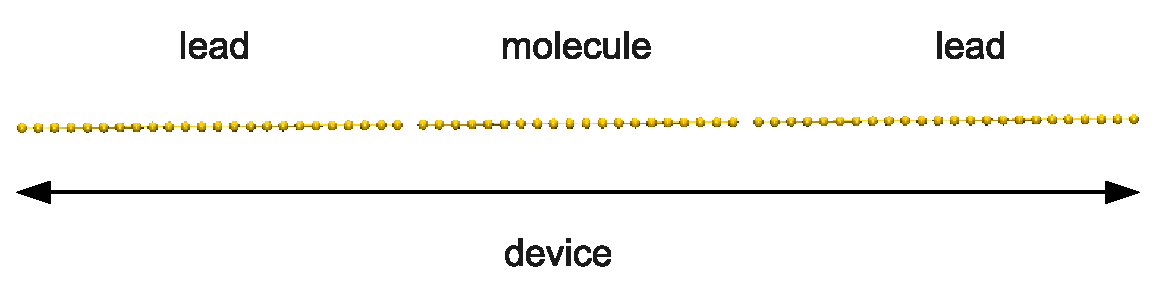
\includegraphics[width=0.9\linewidth]{figures/chaincapdevice}
	\end{center}
	\caption{Model system studied in this work. The molecule consists of
        20 Gold atoms, while the explicit electrode regions each consist of 24
	atoms. The spacing between molecules and electrodes determines the
	coupling of the molecular states to the electrodes.}
	\label{fig:chaincapdevice}
\end{figure}

The regions outside of the explicit atomic region are described by a
\ac{CAP} in analogy to the use of electrode self-energies. The details of
the ab initio \ac{CAP} used are described below and its use has advantages
when including electron correlations into the calculations. In
zero$^{th}$ order, we use the Hartree-Fock approximation to calculate
quasiparticle states and the transmission spectrum for the model system
is calculated using a Green's function approach as
implemented in the TIMES program~\cite{times} with the electrodes in
these scattering calculations described using standard electrode self-energies.
This scattering calculation delivers the Hartree-Fock quasiparticle
spectrum including the energy shifts and state broadening that arise
from coupling the molecular region to electrodes, and serves as the
reference point for discussing subsequent calculations performed at
different levels of approximation.

% Isn't it a bit strange to emphasize HF as the 0th order approximation
% when we decided that the single determinant QP spectrum (with wider peaks
% than Koopmans) was not something we wanted to dwell on?

\subsection{Complex Absorbing Potential}
\label{subsec:CAP}

To treat electron correlations, we apply the method of \ac{CI}. The \ac{CI}
method is the application of the Rayleigh-Ritz linear variational principle
to the calculation of quantum many-electron energies. Within this approach,
the many-electron wavefunction is expanded in terms of Slater determinants
(or spin-coupled sums of determinants referred to as \acp{CSF}). Variation
of the \ac{CI} expansion coefficients leads to a matrix eigenvalue problem
\begin{equation}
\um{H} \vec{c} = E \um{S} \vec{c},
\end{equation} 
where $\um{H}$ is the matrix representation of the many-electron
Hamiltonian in the CSF basis, $\um{S}$ is the metric for the CSF basis,
$E$ is a many-electron energy and $\vec{c}$ is the vector of the
expansion coefficients or CI vector. The matrix elements of $\um{H}$
and $\um{S}$ are constructed from one- and two-electron integrals
defined in the single particle basis used to construct the CSFs, and for
example can be Hartree-Fock states. However, in the CI treatment of the
many-electron problem, no reference is made to single particle or
quasiparticle energies. Hence the inclusion of the electrodes into the
CI problem using electrode self-energies is complicated by the fact that
the self-energies are functions of the quasiparticle energies on the
electrodes. To avoid this complication, we employ instead energy-independent
\acp{CAP} that serve as replacement to the self-energy terms, eliminating
reference to single particle energies into the resulting \ac{CI}
problem~\cite{muga2004, henderson, riss_meyer}.
Note however, that by opening the system using either electrode self-energies
or \acp{CAP},  the traditionally Hermitian \ac{CI} generalized eigenvalue
problem becomes a complex symmetric generalized eigenvalue problem. The
procedure for construction of an energy-independent \ai \ac{CAP} from the
energy-dependant self-energy is discussed in detail in ref.~\cite{henderson}.
We briefly cover the essential points needed for the generation of the
\ac{CAP} in the following.

We first consider two electrodes described by known left ($\Sigma_L(\omega)$)
and right ($\Sigma_R(\omega)$) self-energies. In practice, the complex valued
self-energies for the electrodes are calculated using the TIMES
program~\cite{times}. These self-energies are added to the device region
Hamiltonian $\um{H}_D$ to yield
\begin{subequations}
\begin{align}
        [\um{H}_D + \lambda \um{\Sigma_L}(\omega_i^\lambda)
            +\lambda \um{\Sigma_R}(\omega_i^\lambda)] \ket{U_i^\lambda}
        &= \omega_i^\lambda \ket{U_i^\lambda} \\
        \bra{V_i^\lambda} [\um{H}_D + \lambda \um{\Sigma_L}(\omega_i^\lambda)
            +\lambda \um{\Sigma_R}(\omega_i^\lambda)]
        &= \omega_i^\lambda \bra{V_i^\lambda},
        \label{eq:adiabaticap}
\end{align}
\end{subequations}
where the parameter $\lambda$ is introduced to allow for an adiabatic
coupling between the electrode states and the extended device region
'molecular states'.  At $\lambda = 0$, the states on the extended device
region are obtained as described by eigenvectors $\ket{X_i}$ (that may
be chosen real) and real eigenvalues $\varepsilon_i$. As $\lambda$ is
increased the device region and electrode single particle states begin
to couple until at $\lambda=1$, the Hartree-Fock states for the open
system are given by the complex energies $\omega_i$, right eigenvectors
$\ket{U_i}$ and left eigenvectors $\bra{V_i}$; the left and right
eigenvectors are a consequence of introducing the complex valued
self-energies into the eigenvalue problem. The introduction of the
adiabatic coupling of the self-energies permits us to 'label' the
molecular states and to follow their evolution as the system is opened.
This allows us to use the prescription given in the following to
calculate an \ai \ac{CAP} by selecting those eigenvalues that correspond
to the uncoupled device region states. At $\lambda=1$, the real part of
$\omega_i$ gives the energy of the $i$th resonance including the shift due
to electrode coupling and the imaginary part gives the level broadening.

The goal is to build an energy-independent complex potential
$\um{W} = \um{W_L} + \um{W_R}$
such that the Hamiltonian $\um{H}_D + \um{W}$ has the same eigenvalues
as when calculated using the explict self-energies. Such a Hamiltonian is
not readily constructed as when we select the different $\omega_i$, we are
as a consequence selecting different Hamiltonians
$\um{H}_D + \um{\Sigma_L}(\omega_i) + \um{\Sigma_R}(\omega_i)$
and the biorthogonality for the left and right eigenvectors does not
necessarily hold ($<V_i|U_j> \ne \delta_{ij}$). We consider instead
constructions which yield eigenvalues that approximate the $\omega_i$  and
eigenvectors that approximate the left and right eigenvectors while
satisifying biorthogonality. Given such a set of approximate eigenvectors
we write
\begin{equation}
    \um{W} = \sum_i  \ket{U^\prime_i} \omega_i \bra{V^\prime_i} - \um{H}_D
    \label{eq:capsdefUV}
\end{equation}
which for biorthogonal $\ket{V^\prime_i}$ and $\bra{U^\prime_i}$ will by
construction give an operator $\um{H}_D + \um{W}$ with the correct eigenvalues
and approximate eigenvectors. In practice we work in the real basis of the
device region and calculate
\begin{equation}
    \um{W} = \um{S} \um{X} \um{\omega}\um{X}^\dagger - \um{H}_D
    \label{eq:capsdefX}
\end{equation}
in matrix form, with $\um{S}$ the overlap or metric for the atomic
orbital basis used to describe the device region, $\um{X}^\dagger$ and
$\um{X}$ are the matrices of the eigenvectors of device region
Hamiltonion $\um{H}_D$, and $\um{\omega}$ is the eigenvalue matrix calculated
at $\lambda = 1$. In practice, as the self-energies are independent of the
device region for a properly defined 'extended device region', the \acp{CAP}
are generated on the electrodes and then transformed to the molecular orbital
basis of the device region.

% This projection introduces a small amount of inaccuracy, as will be discussed
% later.

When applying this approximation to generation of the \ac{CAP}, a
comparison can be performed against the energy level shifts and broadening
obtained from explicit calculations using the self-energy. To accomplish
this comparison, we first calculate the electron transmission through
the device region using the Green's function
approach. The calculation is then repeated but in the definition of the
Green's function $G$ and spectral densities $\Lambda_{L/R}$ the
self-energy terms are replaced with the \acp{CAP} $\um{W}_{L/R}$ leading
to the following expressions:
\begin{subequations}
  \begin{align}
	  \um{G}^{-1} &= [E\um{S}_0 - (\um{H}_0 + \um{W})], \\
	  \um{\Lambda}_{(L/R)} &= i \left( \um{W}_{(L/R)} - \um{W}^\dagger_{(L/R)}
    \right).
  \end{align}
  \label{eq:glambdadef}
\end{subequations}
The transmission is then calculated as
\begin{equation}
  T = \um{Tr} \left[ \um{\Lambda}_L \um{G} \um{\Lambda}_R \um{G}^\dagger \right]
  \label{eq:transmfromG}
\end{equation}
with the \acp{CAP} playing the role of the electrode self-energies.
The comparison obtained in this manner is shown in
fig.~\ref{fig:transdat} revealing that the \ac{CAP} provides an
accurate energy-independent representation of the self-energies and in
particular, good agreement is achieved on the energy range around the
\ac{HOMO}-\ac{LUMO} gap of interest for subsequent investigations.

\begin{figure} 
	\begin{center}
		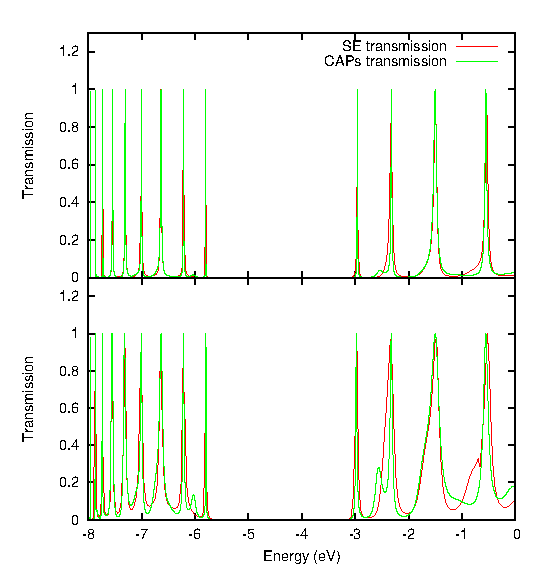
\includegraphics[width=0.9\linewidth]{figures/transdat.eps}
	\end{center}
	\caption{Transmission through the 0.45 nm (top) and 0.40 nm (bottom)
	         systems. The red curve is a transmission spectrum obtained
		 using a conventional self-energy, the green curve is obtained
		 using a \ac{CAP}.}
	\label{fig:transdat}
\end{figure}

\subsection{Complex Symmetric \ac{CI} Problem}

All \ac{CI} calculations  performed use a version of the \ac{MCCI}
program~\cite{mcci1995, mcci1998} modified to treat the complex
symmetric generalized eigenvalue problem that arises when adding the
\ac{CAP} as a one-body operator to the many-electron Coulomb
Hamiltonian used to describe the extended device region and its
interaction with the elecrodes. \ac{MCCI} uses a Lanczos method for
matrix diagonalization and in the newest version of the program the
projection method outlined in ref.~\cite{tarantelli_csd} is introduced to
solve the complex symmetric generalized eigenvalue problem. \ac{MCCI}
computes energy estimates by an iterative process, starting from a set
of \acp{CSF} (which initially may be a single \ac{CSF}).
Relative to the trial vector, additional \acp{CSF} are randomly
generated by single and double excitations relative the \acp{CSF} in the
trial vector. The \ac{CI} matrix diagonalization problem is solved on
the subspace defined by the resulting expanded vector. This vector is
then screened or 'pruned' by removing \acp{CSF} whose associated coefficient
in the \ac{CI} eigenvector has a magnitude lower than a given coefficient
threshold. This 'pruned' vector serves as trial vector for the generation of
a new set of randomly generated \acp{CSF}, and this sequence is repeated until
convergence in the energy and CI vector length is reached. Details of the
\ac{MCCI} method may be found in refs.~\cite{mcci1995,mcci1998,mcci2000,multiref}.

The use of \ac{MCCI} in the present study allows us to follow the
evolution of quasiparticle energies as electron correlations are
increased; this is achieved by starting from a single determinant picture
and then systematically including important electron correlations by
performing \ac{CI} calculations at different values of the coefficient
selection threshold. As the coefficient selection threshold is reduced,
more \acp{CSF} are included in the calculations leading to a more highly
correlated model.

\subsection{Quasiparticle Energies}

From a many-electron standpoint, energy differences between
many-electron states determine quasiparticle excitations, as well as
electron affinities and ionization energies, or addition and substraction
energies respectively. In this study, we focus on the electron
affinities and ionization potentials of the {\it explicit} device
region. For example, the electron affinity is given by the
difference in energies for the $N$-electron state $E^N$ and the
$(N+1)$-particle state $E^{N+1}$
\begin{equation}
\omega_{\rm EA} = E^{N+1} -E^N,
\end{equation}
and similarly the ionization potential
\begin{equation}
\omega_{\rm IP} =  E^N - E^{N-1}
\end{equation}
is the energy difference between the $N-1$ and $N$ many-electron states.
Through the introduction of \acp{CAP}, the device region becomes an open
system resulting in complex many-electron energies. Hence the
quasiparticles energies $\omega$ are complex. It is the real energy
shift and imaginary lifetime due to the opening of the system, as well
as due to the introduction of electron correlations, which we study for
the molecular device states.
From the transmission calculations on our model using a scattering Green's
function approach, the transmission of the states that evolve from the
uncoupled device states is determined. It is found that these states have
transmission values close to unity and their lineshapes can be roughly
approximated by a Lorentzian profile (there is some indication of Fano-type
resonances indicating that there is a degree of coupling between 
electrodes, but these small effects do not influence our analysis). Thus in
order to compare to transmission spectra obtained from the
single-particle scattering Green's function calculations picture, we construct
Lorentzian peaks from the complex quasiparticles $\omega_i$:
\begin{equation}
        f(\varepsilon;\omega_i)
        = \frac{\left( \Gamma/2 \right)^2}
               {(\varepsilon - \operatorname{Re}(\omega_i))^2
               + \left( \Gamma/2 \right)^2}
        \label{eq:lobro}
\end{equation}
where $\Gamma = 2 \operatorname{Im}(\omega_i)$ is the lifetime of the
quasiparticle (i.e., the width of the Lorentzian peak).

\section{Results and Discussion}
\label{sec:results}

\subsection{\ac{CAP} Validation}
\label{subsec:SingleParticle}

As a validation of our approach, we first consider if
the \ac{CAP} as generated according to the method given in
section~\ref{subsec:CAP} results in the correct complex single-particle
eigenvalues.
For comparison we construct Lorentzian peaks determined by the complex
eigenvalues obtained for the \acp{CAP}, and compare to the transmission
spectrum of the device obtained using explicit self-energies and a scattering
calculation; the results of the comparison are shown in fig.~\ref{fig:13evals}.
This is a case of weak coupling, as can be seen by the narrowness of the
transmission peaks, and by the fact that they are not significantly shifted
from the real-valued Hartree-Fock single-particle levels. %Jim wants this out?
The agreement between the Green function transmission (red) and the peaks
derived from the eigenvalues of $\um{H}_0 + \um{W}$ (green) is excellent,
both in terms of position (real part) and width (imaginary part). In the inset,
the region around the \ac{HOMO} is plotted in detail, showing the extent of
the agreement between the two approaches (the green and red curves effectively
overlap for the energy scales we will consider).

\begin{figure} 
	\begin{center}
		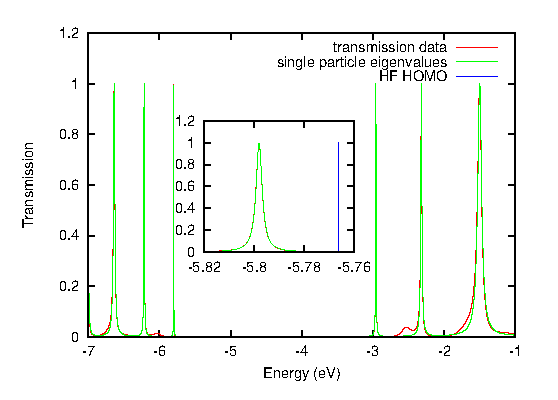
\includegraphics[width=0.9\linewidth]{figures/13evals}
	\end{center}
	\caption{Comparison of transmission data (red) with Lorentzian
	broadened complex eigenvalues of $\um{H}_0 + \um{W}$ (green) for a
	model system as described in section~\ref{subsec:modelsystem}, with
	device-lead gap of 0.45 nm. Transmission data was obtained from
	scattering calculations using a Green's functions formalism and
	explicit electrode self-energies.
	The inset shows a close-up view of the \ac{HOMO}, with the HF \ac{HOMO}
	shown in blue for reference.
	}
	\label{fig:13evals}
\end{figure}

\section{Many-Body Analysis}

We start our analysis by considering the more weakly coupled system (45
nm separation). The transmission curves obtained for the \ac{HOMO} at
different levels of theory are plotted in figure~\ref{fig:all45A}. Firstly,
we can represent the wave function as a single determinant. Since the
only difference between this and the single particle case described above
is the basis, it is not surprising to see good agreement, especially in
the position of the peak. Next, we can approximate the wave function by
taking the same reference determinant as above, and also including all
of its single excitations. We can expect that the results from this are
analogous to a delta-SCF procedure, since by Thouless' theorem
\cite{Thouless} this can be described as a single determinant in a
different basis. Finally, we can include more correlations by running
the mcci procedure, first at cmin=3e-3, and then at cmin=1e-3, which
generally corresponds to moderate correlation. As expected from chemical
intuition, CI singles gives the smallest gap and single determinants the
largest, with the correlated peaks in the middle and the gap closing with
increasing correlation. The width of the peaks in the different many-body
approximations stays nearly constant, implying that broadening (in this
case corresponding to a state lifetime of approximately
$7 \times 10^{-14}$ s for the \ac{HOMO} and $3 \times 10^{-14}$ s for
the \ac{LUMO}) is accurately captured at the SCF (single determinant)
level for this system.

\begin{figure}
	\begin{center}
		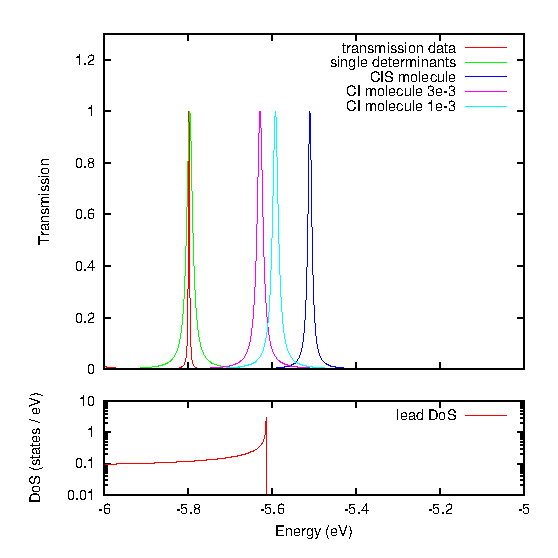
\includegraphics[width=0.9\linewidth]{figures/all45A.eps}
	\end{center}
	\caption{''Molecule'' cmcci peaks (45A system)}
	\label{fig:all45A}
\end{figure}

We now repeat the analysis for the more strongly coupled system, results
of which are plotted in figure~\ref{fig:all40A}. The same picture emerges,
with the CI singles case having the smallest gap, and the single determinant
the largest, although at the \ac{HOMO} now the weakly correlated (cmin=3e-3)
case overlaps with the single determinant case. However, when decreasing
the cmin parameter (increasing correlation), the peak shifts back up,
reducing the gap. With respect to the broadenings, we see a similar
picture as for the previous system; increasing correlation has no
significant effect on the level broadening.

\begin{figure}
	\begin{center}
		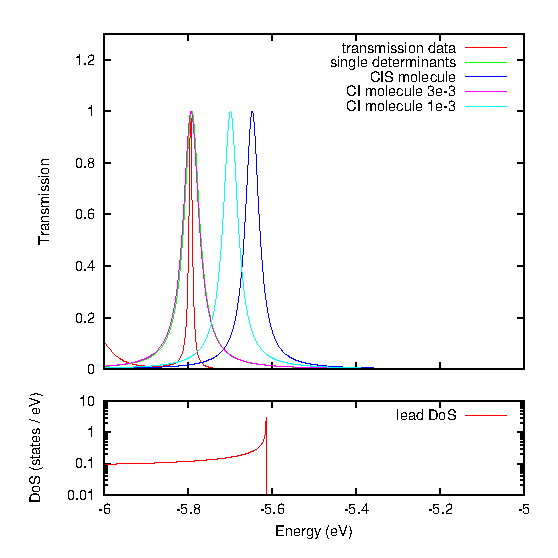
\includegraphics[width=0.9\linewidth]{figures/all40A.eps}
	\end{center}
	\caption{''Molecule'' cmcci peaks (40A system)}
	\label{fig:all40A}
\end{figure}

Finally, we investigate the effect of including excitations on the leads.
Until this point, we have always constrained our CI space to \acp{CSF}
which represent excitations from and to orbitals localized on the molecule.
Lead excitations have been previously shown to have significant effects
on current flow through two-level model systems
\cite{galperin_nitzan2006leadexcitations}. 
The first notable feature in this case (see figure~\ref{fig:cidevregion})
is found in the CI singles case, where the \ac{LUMO} peak is much broader
than all other peaks studied (state lifetime of $5 \times 10^{-15}$ s).
This can be directly related to the fact that the $N+1$-electron state
contains two (instead of one) significant CSFs, one of which has the extra
electron in a lead orbital (This does not happen in any of the other cases
we studied).

Upon including more CSFs with the mcci procedure, we see a quantitative
difference from the ''molecule'' analysis above; the QP gap widens, mainly
due to the rising of the \ac{LUMO} up to around $-2.5$ eV in both systems.
Also, the broadness of the \ac{LUMO} peak for the 4.0A separated system
is mitigated in the CI calculation (leading to a lifetime of
$1 \times 10^{-17}$ s). This can be traced back to the fact that we go
back to having only one significant CSF in the associated $N+1$-electron
CI vector.

\begin{figure}
	\begin{center}
		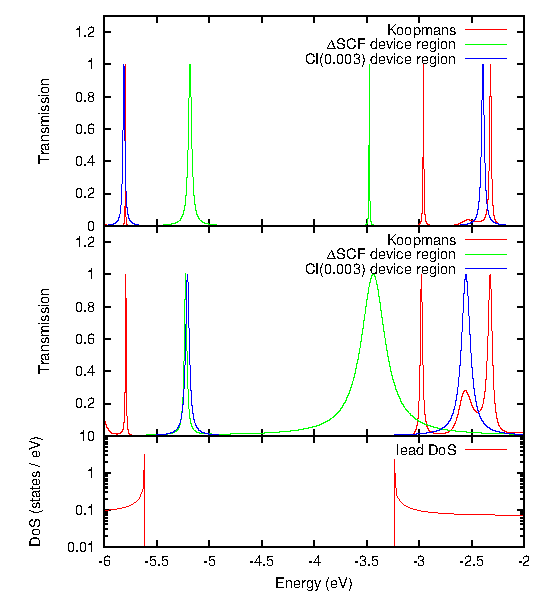
\includegraphics[width=0.9\linewidth]{figures/cidevregion.eps}
	\end{center}
	\caption{CI for the \ac{LUMO} of the 0.45 (top) and 0.40 nm (middle)
                 systems, with the Density of States of the leads plotted
                 below.}
	\label{fig:cidevregion}
\end{figure}

\section{Conclusions}
\label{sec:conclusions}

In this work we presented the results of the application of wavefunction
methods to the study of semi-infinite systems using a \ac{CAP}. It was shown
that when lead exitations are not included, the QP gap is smaller than in the
HF case, and becomes smaller as more correlation is included. Inclusion of
lead excitations decreases the gap in the CI Singles case, but increases it
substantially in the more correlated CI cases.

The ability to accurately describe these QP levels (which in this case
correspond to \ac{IP} and \ac{EA}) has been shown to be closely related to an
accurate description of transport~\cite{golden}. This work opens the door for
the application of non-empirical wave funcion methods to the study of quantum
transport in nanoscale systems in which the lifetime broadening is captured
accurately by a self-energy-derived \ac{CAP}.
